\section{Результаты работы}

После запуска программы выводится меню c 19 пунктами (рис.~\ref{fig:menu}).

\begin{figure}[H]
	\centering
	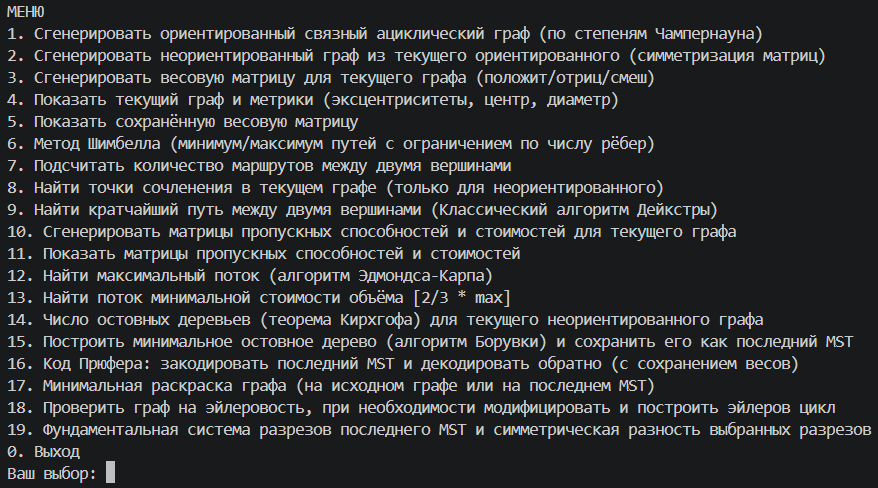
\includegraphics[width=0.9\textwidth]{pic/menu.png}
	\caption{Вывод меню программы}
	\label{fig:menu}
\end{figure}

При вводе 1, происходит генерация ориентированного связного графа по введённым пользователем количеству вершин (рис.~\ref{fig:gen}).

\begin{figure}[H]
	\centering
	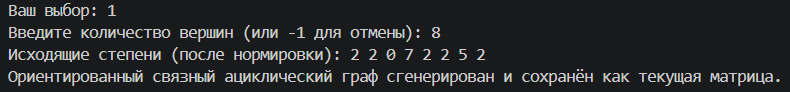
\includegraphics[width=0.9\textwidth]{pic/generation.png}
	\caption{Генерация графа}
	\label{fig:gen}
\end{figure}

На рис.~\ref{fig:neor} представлена генерация неориентированного графа из текущего ориентированного.

\begin{figure}[H]
	\centering
	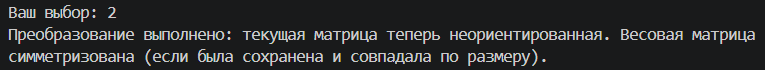
\includegraphics[width=0.9\textwidth]{pic/gen_neor.png}
	\caption{Генерация неориентированного графа}
	\label{fig:neor}
\end{figure}

На рис.~\ref{fig:vesa} представлена генерация весовой матрицы с настройкой весов: положительные, отрицательные и смешанные.

\begin{figure}[H]
	\centering
	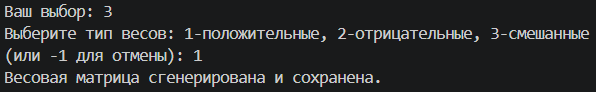
\includegraphics[width=0.9\textwidth]{pic/vesa.png}
	\caption{Генерация весовой матрицы}
	\label{fig:vesa}
\end{figure}

На рис.~\ref{fig:metrics} показан вывод матрицы смежности текущего графа и его метрик.

\begin{figure}[H]
	\centering
	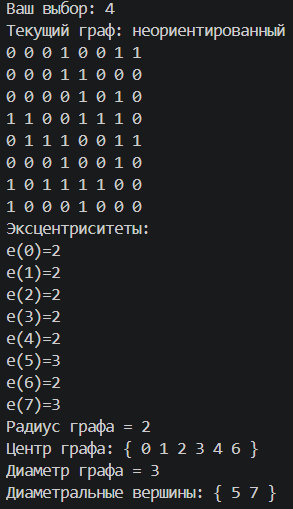
\includegraphics[width=0.8\textwidth]{pic/metrics.png}
	\caption{Вывод матрицы смежности и метрик}
	\label{fig:metrics}
\end{figure}

На рис.~\ref{fig:vesa_mat} представлен вывод сохранённый весовой матрицы.

\begin{figure}[H]
	\centering
	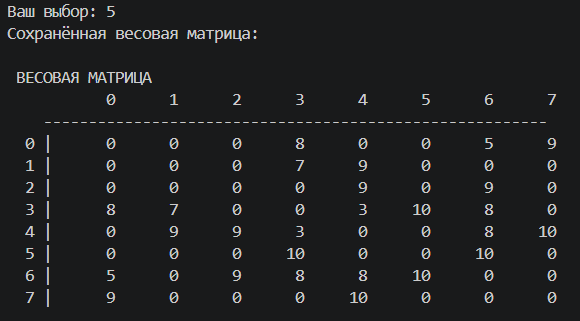
\includegraphics[width=0.9\textwidth]{pic/vesa_mat.png}
	\caption{Вывод весовой матрицы}
	\label{fig:vesa_mat}
\end{figure}

На рис.~\ref{fig:shimbell} показан метод Шимбелла.

\begin{figure}[H]
	\centering
	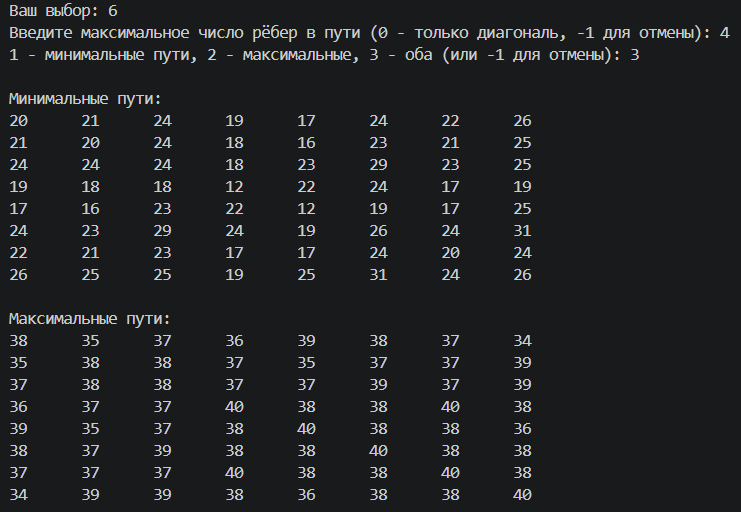
\includegraphics[width=0.9\textwidth]{pic/shimbell.png}
	\caption{Метод Шимбелла}
	\label{fig:shimbell}
\end{figure}

На рис.~\ref{fig:marsh} представлен вывод количества маршрутов между заданными вершинами.

\begin{figure}[H]
	\centering
	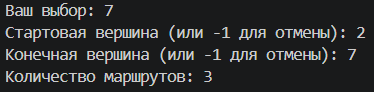
\includegraphics[width=0.9\textwidth]{pic/marsh.png}
	\caption{Поиск колисчества маршрутов}
	\label{fig:marsh}
\end{figure}

На рис.~\ref{fig:sochlen} приведён поиск точек сочленения в неориентированном графе.

\begin{figure}[H]
	\centering
	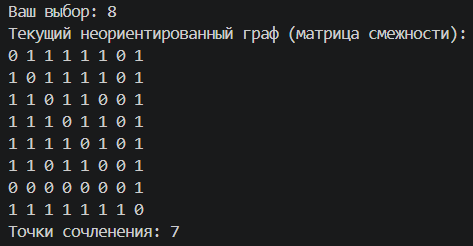
\includegraphics[width=0.9\textwidth]{pic/sochlen.png}
	\caption{Поиск точек сочленения}
	\label{fig:sochlen}
\end{figure}

На рис.~\ref{fig:dejcstra} показан алгоритм Дейкстры.

\begin{figure}[H]
	\centering
	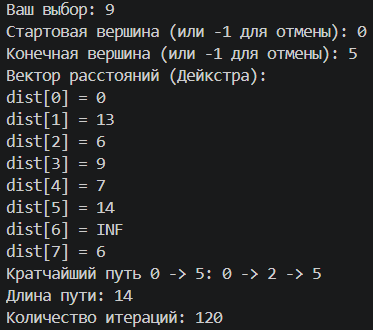
\includegraphics[width=0.9\textwidth]{pic/dejcstra.png}
	\caption{Вывод результатов алгоритма Дейкстры}
	\label{fig:dejcstra}
\end{figure}

На рис.~\ref{fig:prop_cost} представлена генерация матриц пропускных способностей и стоимостей.

\begin{figure}[H]
	\centering
	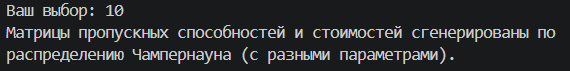
\includegraphics[width=0.9\textwidth]{pic/prop_cost.png}
	\caption{Генерация матриц пропускных способностей и стоимостей}
	\label{fig:prop_cost}
\end{figure}

На рис.~\ref{fig:mat_prop_cost} показан вывод матриц пропускных способностей и стоимостей.

\begin{figure}[H]
	\centering
	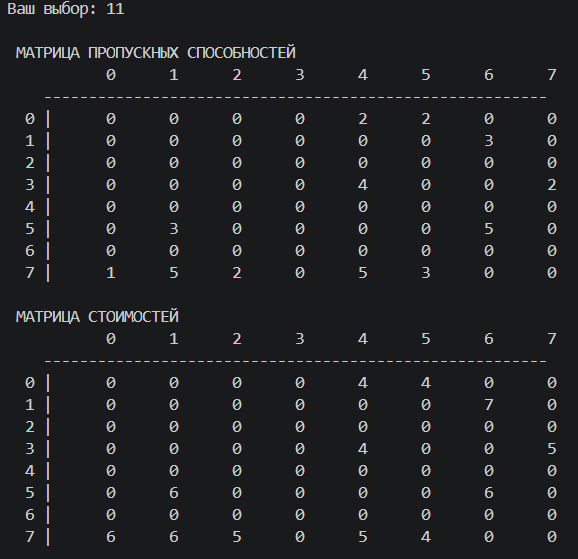
\includegraphics[width=0.9\textwidth]{pic/mat_prop_cost.png}
	\caption{Вывод матриц пропускных способностей и стоимостей}
	\label{fig:mat_prop_cost}
\end{figure}

На рис.~\ref{fig:max_potok} представлен поиск максимального потока.

\begin{figure}[H]
	\centering
	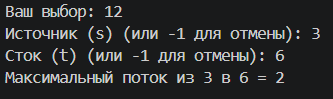
\includegraphics[width=0.9\textwidth]{pic/max_potok.png}
	\caption{Поиск максимального потока}
	\label{fig:max_potok}
\end{figure}

На рис.~\ref{fig:min_stoim_potok} показан поиск потока минимальной стоимости.

\begin{figure}[H]
	\centering
	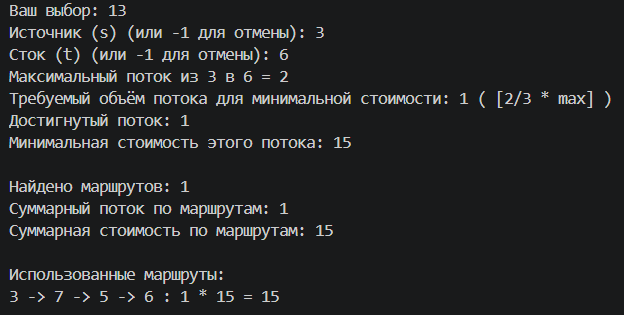
\includegraphics[width=0.9\textwidth]{pic/min_stoim_potok.png}
	\caption{Поиск потока минимальной стоимости}
	\label{fig:min_stoim_potok}
\end{figure}

На рис.~\ref{fig:ostov} показан поиск количества остовных деревьев по теореме Кирхгофа для неориентированного графа.

\begin{figure}[H]
	\centering
	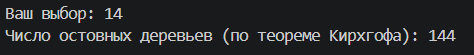
\includegraphics[width=0.9\textwidth]{pic/ostov.png}
	\caption{Теорема Кирхгофа}
	\label{fig:ostov}
\end{figure}

На рис.~\ref{fig:mst} представлено построение минимального остовного дерева по алгоритму Борувки.

\begin{figure}[H]
	\centering
	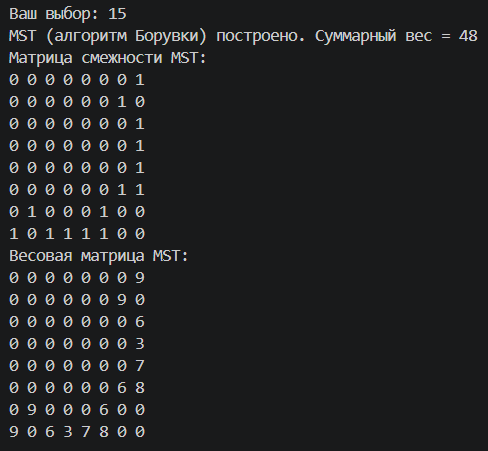
\includegraphics[width=0.9\textwidth]{pic/mst.png}
	\caption{Построение минимального остовного дерева}
	\label{fig:mst}
\end{figure}

На рис.~\ref{fig:prufer} показано кодирование и декодирование минимального остовного дерева кодом Прюфера.

\begin{figure}[H]
	\centering
	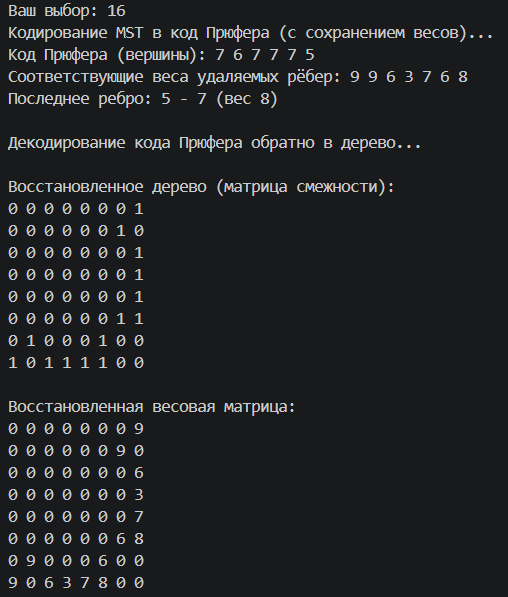
\includegraphics[width=0.9\textwidth]{pic/prufer.png}
	\caption{Код Прюфера}
	\label{fig:prufer}
\end{figure}

На рис.~\ref{fig:color} представлен алгоритм минимальной раскраски графа.

\begin{figure}[H]
	\centering
	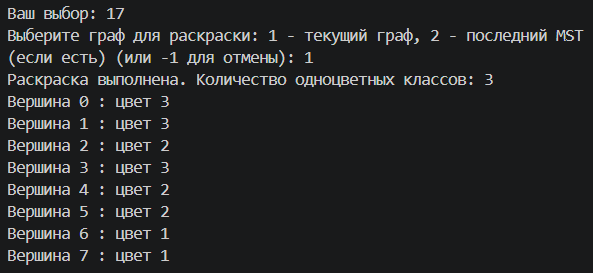
\includegraphics[width=0.9\textwidth]{pic/color.png}
	\caption{Минимальная раскраска графа}
	\label{fig:color}
\end{figure}

На рис.~\ref{fig:euler} показана проверка графа на эйлеровость и его дальнейшая модификация.

\begin{figure}[H]
	\centering
	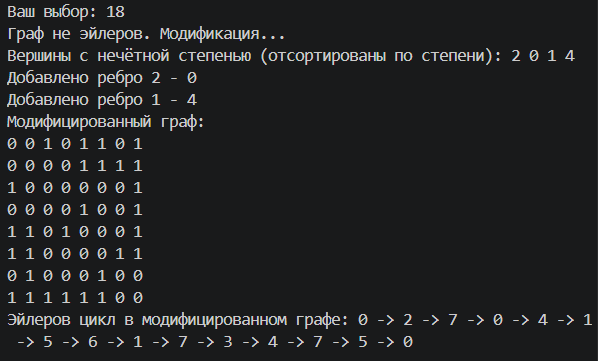
\includegraphics[width=0.9\textwidth]{pic/euler.png}
	\caption{Эйлеровы графы}
	\label{fig:euler}
\end{figure}

На рис.~\ref{fig:razrez} представлено нахождение фундаментальной системы разрезов и их симметрическая разность.

\begin{figure}[H]
	\centering
	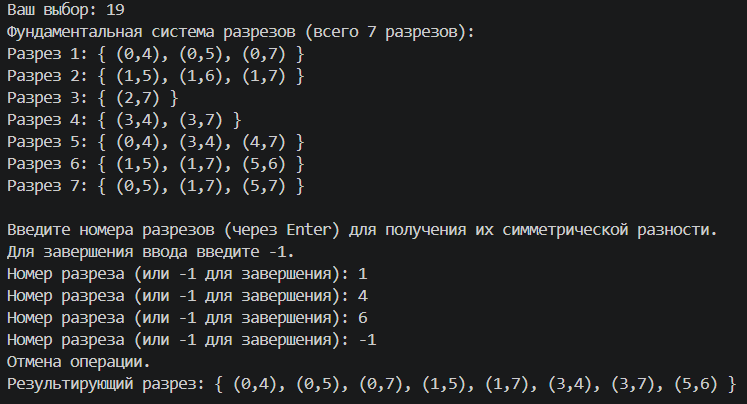
\includegraphics[width=0.9\textwidth]{pic/razrez.png}
	\caption{Фундаментальная система разрезов}
	\label{fig:razrez}
\end{figure}